\documentclass[a4paper,10pt]{article}

\usepackage[left=3.5cm, right=3.5cm]{geometry}

\usepackage{ngerman}
\usepackage[utf8]{inputenc}

\usepackage{graphicx}

\usepackage[index,nonumber,contents]{cuisine}

% Some styling of the recipe
%\RecipeWidths{Total}{Number of servings}{Number}{Ingredient}{Quantity}{Units}
\RecipeWidths{\textwidth}{3cm}{0.5cm}{3.75cm}{1.cm}{1.75cm}

\renewcommand*{\recipetitlefont}{\large\bfseries\sffamily}
\renewcommand*{\recipequantityfont}{\sffamily\bfseries}
\renewcommand*{\recipeunitfont}{\sffamily}
\renewcommand*{\recipeingredientfont}{\sffamily}
\renewcommand*{\recipefreeformfont}{\itshape}

% Images are stored here
\graphicspath{{./images/}}

% Draw frame around images
\setlength\fboxsep{0pt}
\setlength\fboxrule{0.5pt}

% Give credit
\newcommand{\creator}[2][von]{\textnormal{\small{(#1 #2)}}}

% Don't number sections but display them in the TOC
\setcounter{secnumdepth}{0}

\title{\Huge Vegan Weitersegeln}
%\author{Claudia Wildner, Tobias Timmler, Daniel Kreischer, Nicole Stoffels}

\begin{document}

    \maketitle
    \begin{center}
         \fbox{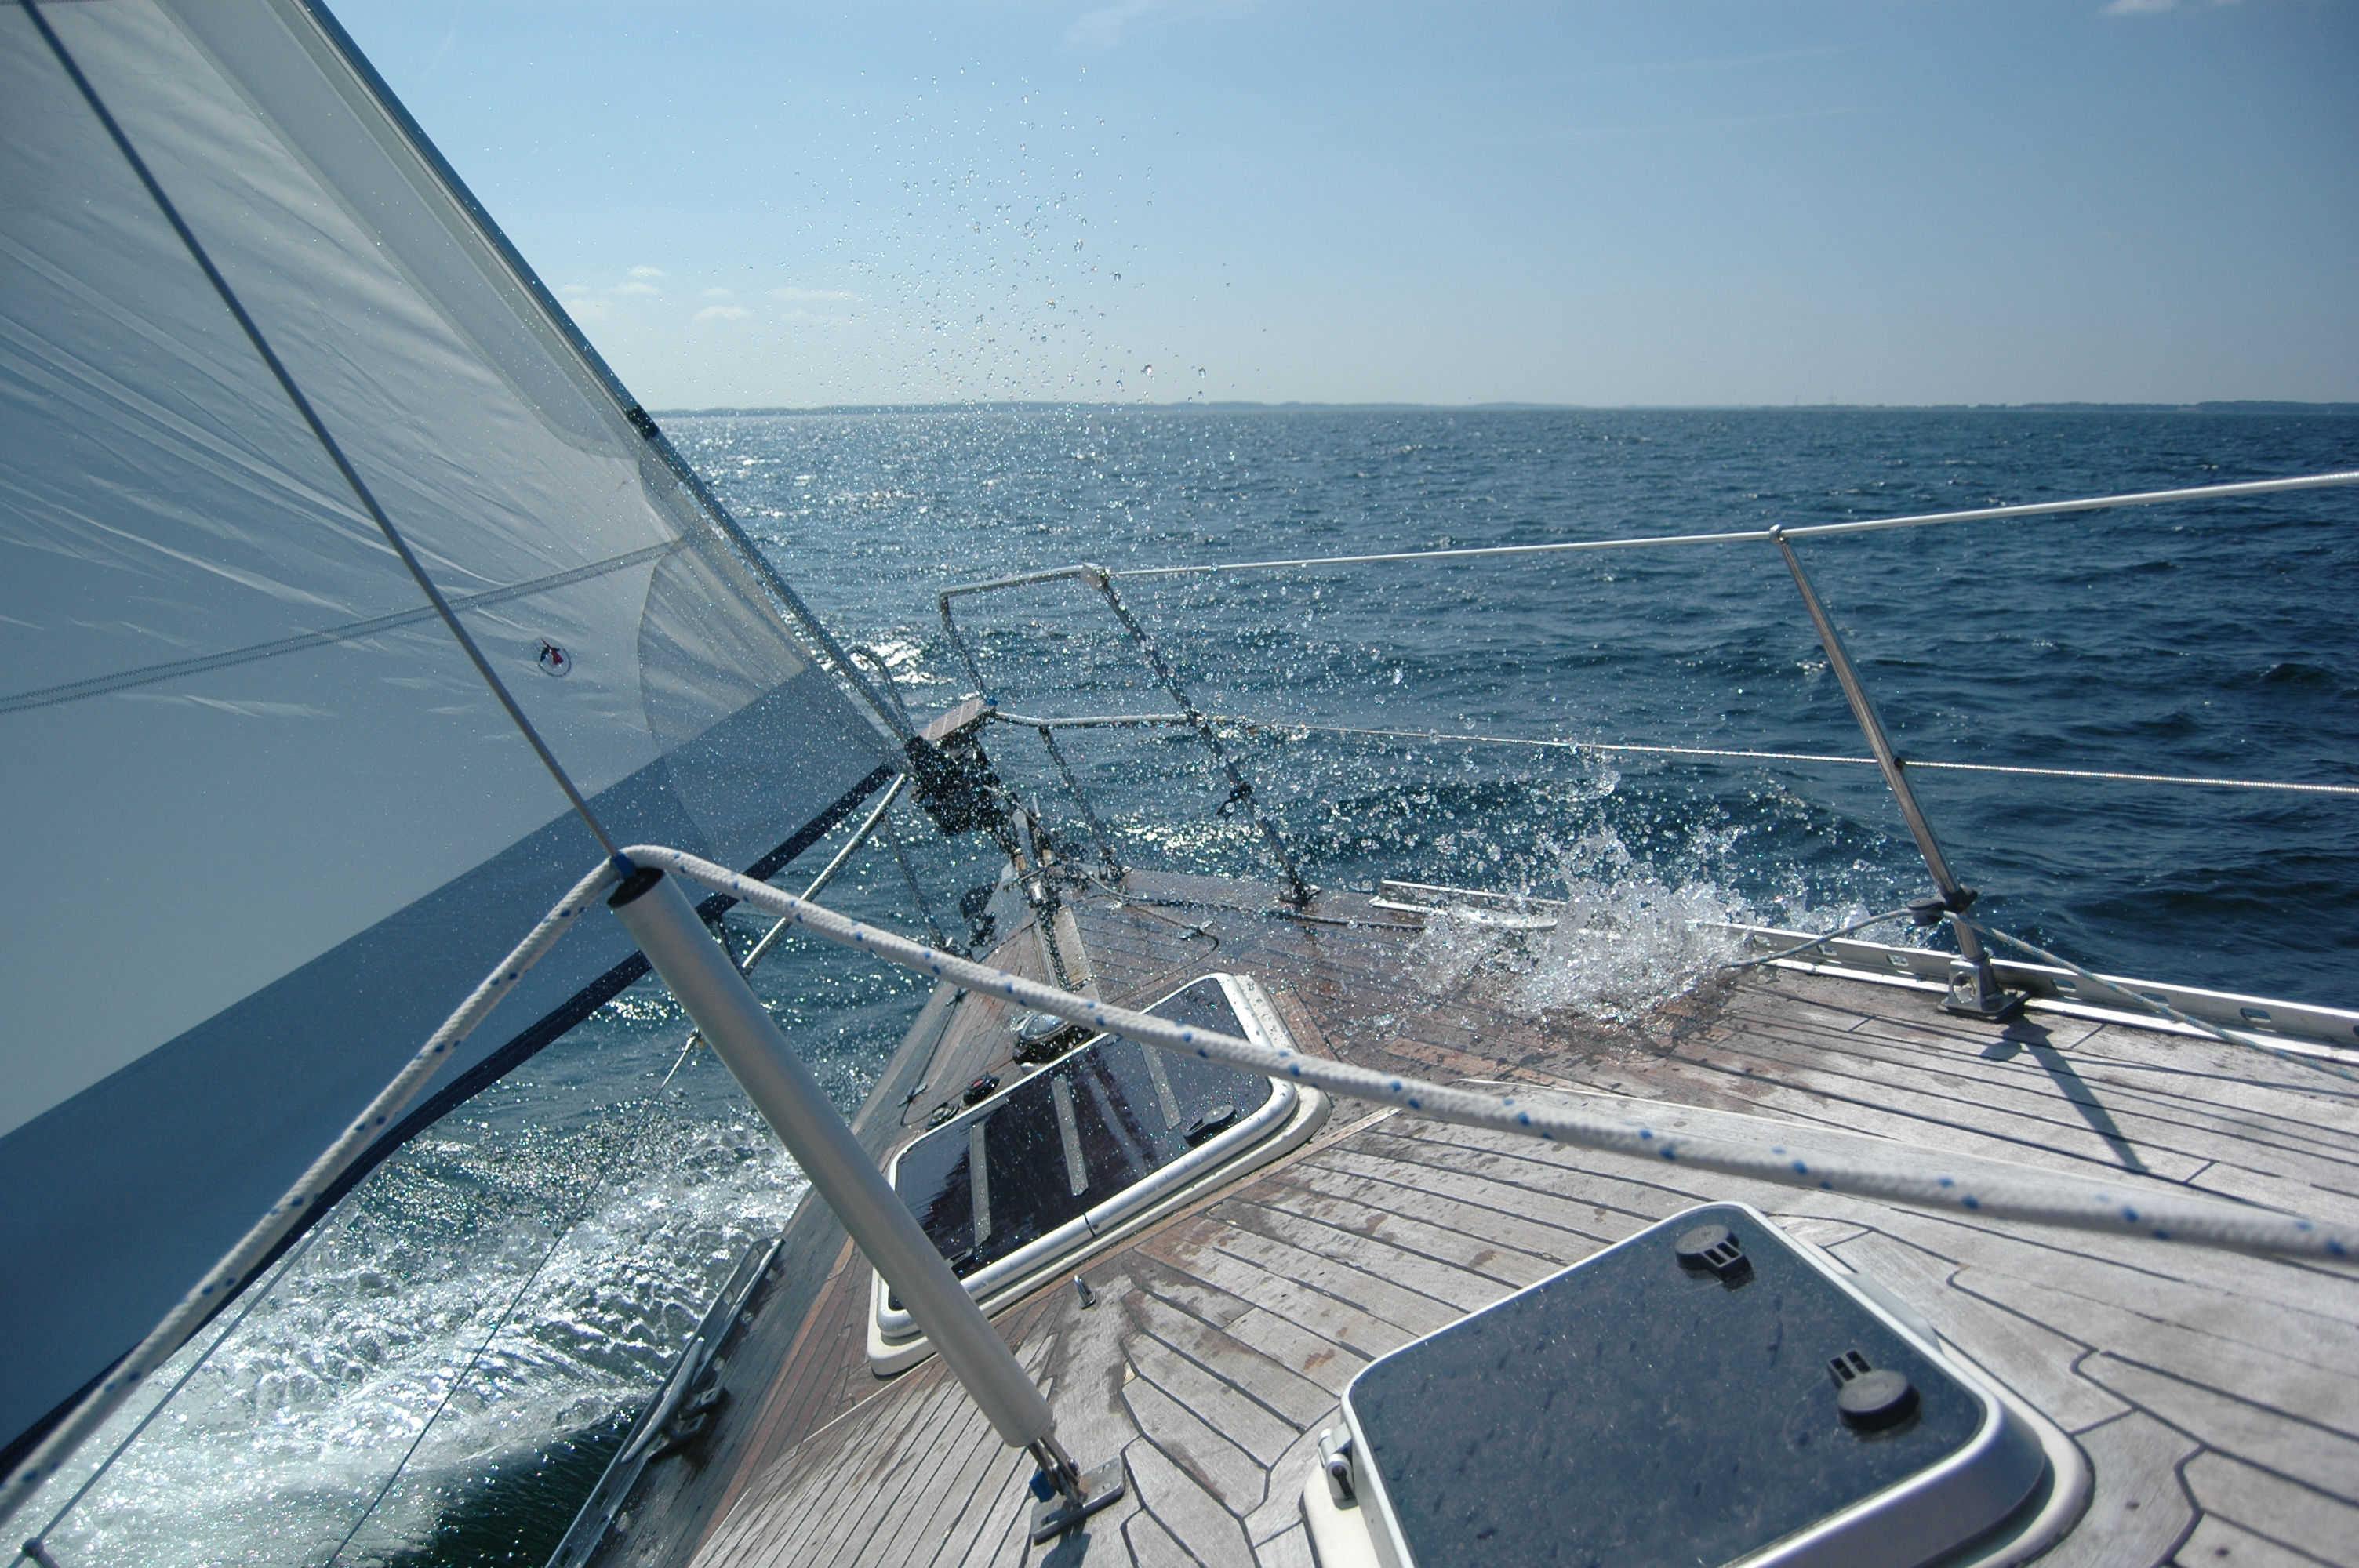
\includegraphics[width=150mm]{Bilder/cover}}
    \end{center}
    \thispagestyle{empty}
    \newpage

    \tableofcontents
    \newpage


    \section{Frühstück}

    \begin{recipe}{Espresso Gelee}{Für 6 bis 8 Gläser}{Ca. 30 Minuten}
        
        \freeform \hfill 
        \fbox{\includegraphics[width=64mm]{Bilder/espressogelee}}
        
        \ingredient[150]{g}{Zartbitterschokolade}
            Schokolade fein hacken und ins Gefrierfach stellen.
        \ingredient[1]{}{Vanilleschote}
            Vanilleschote ausschaben.
        \ingredient[900]{ml}{frisch gekochter Espresso}
        \ingredient[\fr{1}{4}]{TL}{Zimt}
        \ingredient[500]{g}{Gelierzucker 2:1}
        \ingredient[1]{EL}{Zitronensaft}
            Espresso, Vanille, Zimt, Gelierzucker und Zitronensaft zum Kochen bringen. 4 Minuten leicht kochen.
            5 min abkühlen lassen, dann die Schokolade unterrühren. 
            In die ausgekochten Gläser füllen. Diese sofort verschließen und 5 Minuten auf den Kopf stellen.
        \freeform
            Tipp: Nutzt man Gelierzucker 3:1, die Menge auf 300 g reduzieren. Gelierprobe machen!
    \end{recipe}
   
    \newpage

    \begin{recipe}{Zwiebel-Mett}{Für 10 Portionen}{Ca. 10 Minuten}
        \ingredient[100]{g}{Reiswaffeln}
        \ingredient[1]{große}{Zwiebel}
        Die Reiswaffeln mit den Händen zerbröseln. Zwiebel schälen, fein würfeln und zu den Reiswaffeln geben.
        \ingredient[4]{EL}{Tomatenmark}
        \ingredient[5]{EL}{Gurkensud}
        Das Tomatenmark in 300 ml heißem Wasser auflösen, den Gurkensud hinzugeben. Alles zu den Reiswaffeln 
        hinzufügen.
        \ingredient[]{}{Salz}
        \ingredient[]{}{Pfeffer aus der Mühle}
        Alles gründlich umrühren und mit Salz und Pfeffer abschmecken. Das Mett mindestens 8 Stunden im
        Kühlschrank durchziehen lassen.
        \freeform Der Gurkensud kann auch durch 1 EL Weißweinessig, 1 Prise 
        Zucker und 5 EL Wasser ersetzt werden.
    \end{recipe}
    
    \newpage
    
    \begin{recipe}{Rührtofu}{Für 4 Personen}{Ca. 25 Minuten}
        \ingredient[250]{g}{Räuchertofu}
        \ingredient[8]{EL}{Olivenöl}
        Räuchertofu in kleine Würfel schneiden und mit 2 EL Olivenöl kross 
        anbraten.
        \ingredient[750]{g}{Naturtofu}
        \ingredient[1,5]{TL}{Kurkuma}
        \ingredient[]{}{Salz}
        Naturtofu mit den Händen in eine Schüssel zerbröseln. Mit Kurkuma und 
        Salz würzen. Tofu mit dem restlichen \"Ol scharf anbraten. Dabei nicht 
        zu oft umrühren, damit sich eine leichte braune Kruste bildet.
        \ingredient[400]{g}{Seidentofu}
        \ingredient[1]{Bund}{Schnittlauch}
        \ingredient[]{}{Pfeffer}
        Seidentofu in eine Schüssel geben und grob durchrühren. Wenn der 
        Naturtofu in der Pfanne fertig gebraten ist, Seidentofu drüber geben 
        und eine weitere Minute braten. Rührtofu mit Salz und Pfeffer 
        abschmecken und mit Schnittlauchr\"ollchen bestreuen.
        \freeform Das Salz kann durch Kala Namak ersetzt werden. Das verleiht 
        dem Rührtofu einen Eier-Geschmack.
    \end{recipe}

    \newpage

  
    \section{Salate}
    
    \begin{recipe}{Griechischer Nudelsalat mit Würstchen und Gemüsepuffern}{4 bis 5 Portionen}{}
        \ingredient[1]{Paket}{Vollkornspiralnudeln} 
        Vollkornnudeln in Salzwasser kochen bis sie bissfest sind und in Olivenöl und etwas Nudelwasser schwenken.
        \ingredient[1]{Glas}{grüne kernlose Oliven}
        \ingredient[1]{Glas}{schwarze kernlose Oliven}
        \ingredient[4]{}{Zwiebeln}
        \ingredient[5]{}{Knoblauchzehen}                     
        \ingredient[1]{Paket}{Kirschtomaten}
        Grüne und schwarze Oliven halbieren, Zwiebeln, Knoblauch schälen und klein schneiden. 
        Tomaten vierteln und alles unter die Nudeln heben.
        \ingredient[3]{EL}{vegane Mayonnaise}
        \ingredient[2]{EL}{Senf}
        \ingredient[]{}{Olivenöl}
        \ingredient[1]{}{Zitrone}
        \ingredient[]{}{Cumin}
        \ingredient[]{}{Salz}
        \ingredient[]{}{Pfeffer}
        Aus Mayonnaise, Senf, Olivenöl, Zitrone und Wasser eine Vinaigrette herstellen und mit Salz,
        Pfeffer, Minze und Cumin abschmecken. Die Vinaigrette gerne ein wenig deftiger machen,
        da die Nudeln den Geschmack mildern.
        \ingredient[2 - 3]{Pakete}{Seitanwürstchen}
        \ingredient[1]{Paket}{Gemüsepuffer}        
        \ingredient[]{}{frische Minze}
        Die Gemüsepuffer nach Anweisung auf dem Paket zubereiten und in der Pfanne ausbacken.
        Die Würstchen braten und alles zusammen servieren.
    \end{recipe}

    \newpage    
    
    \section{Suppen}
    
    \begin{recipe}{Kokossuppe mit Süßkartoffeln}{4 - 5 Portionen}{}
        \ingredient[3 - 4]{}{Süßkartoffeln}
        \ingredient[500]{ml}{Gemüsebrühe}
        Die Süßkartoffeln schälen und kleinschneiden. Die Süßkartoffeln in der 
        heißen Brühe 5 Minuten kochen lassen.
        \ingredient[1]{Paket}{Kirschtomaten}
        \ingredient[1]{Bund}{Frühlingszwiebeln}
        \ingredient[2]{Pakete}{Champignons}
        Die Frühlingszwiebeln in Ringe schneiden, die Pilze vierteln und die Tomaten halbieren.
        \ingredient[1]{Bund}{Zitronengras}
        \ingredient[400]{ml}{Kokosmilch}
        \ingredient[1]{Zehe}{Ingwer}
        \ingredient[1]{}{Biozitrone}
        \ingredient[2]{Pakete}{Currypaste}
        Kokosmilch, Zitronengras, Ingwer, Zitronensaft, die Tomaten, die Pilze und die Currypaste zu den
        Süßkartoffel dazu geben und weitere 5 Minuten köcheln. Die Frühlingszwiebeln hinzugeben darin 
        ziehen lassen.
        \ingredient[1]{Bund}{Basilikum (oder auch Koriander)}
        \ingredient[]{}{Salz}
        Mit Salz abschmecken, alles mit Basilikum und/oder Koriander bestreuen, unterheben und servieren.
    \end{recipe}
    
    \newpage
       
    \begin{recipe}{Deftige Linsensuppe}{4 bis 5 Portionen}{}
        \ingredient[1]{Paket}{rote Linsen}
        Die Linsen in reichlich Wasser ohne Salz aufkochen und etwa 15 Minuten köcheln lassen.
        \ingredient[8]{}{große Kartoffeln}
        \ingredient[2]{Bund}{Suppengemüse}
        In der Zwischenzeit die Kartoffeln schälen, in kleine Würfel schneiden, das Suppengemüse putzen 
        und in sehr kleine Würfel schneiden. Das Gemüse zu den Linsen geben und zusammen mit den Linsen kochen.
        \ingredient[2]{Pakete}{passierte Tomaten}
        \ingredient[3 - 4]{EL}{Gemüsebrühe}
        \ingredient[2]{}{Lorbeerblätter}
        Die Lorbeerblätter und das Gemüsebrühepulver hinzugeben. Die passierten Tomaten in die Suppe gießen
        und nach Bedarf mit Wasser auffüllen.
        \ingredient[4]{}{Knoblauchzehen}
        \ingredient[3]{}{Zwiebeln}
        \ingredient[3]{}{Chilischoten}
        Die kleingeschnittenen Zwiebeln, Chilischoten und Knoblauchzehen hinzugeben.
        Die Linsensuppe solange kochen, bis die Kartoffelwürfel weich sind. 
        \ingredient[1]{TL}{Kümmel}
        \ingredient[2]{TL}{Paprikapulver edelsüß}
        \ingredient[]{}{Salz}
        \ingredient[]{}{Pfeffer}
        \ingredient[1]{Bund}{Petersilie}
        \ingredient[]{}{Senf}
        Die gehackte Petersilie hinzufügen und mit Salz, Pfeffer, Senf und wer mag mit reichlich Kümmel abschmecken.
        \ingredient[2]{Pakete}{Räuchertofu}
        \ingredient[2]{Pakete}{Seitanwürstchen}
        Den Räuchertofu kleinschneiden, die Seitanwürstchen in Scheibchen schneiden und in Öl abraten. 
        Beides in die Suppe geben und noch eine Weile bei sehr kleiner Hitze ziehen lassen. 
        \freeform Tipp: Dazu passt wunderbar frisches Baguette oder Ciabatta.
    \end{recipe}
    
    \newpage
    
    
    \section{Hauptgerichte}
    
    \begin{recipe}{Sojageschnetzeltes mit Paprika auf Rotwein}{4 
           - 5 Portionen}{}         
 	\ingredient[2]{Pakete}{grobe Sojaschnetzel}
	Das Sojageschnetzelte 10 Minuten in kochendem Salzwasser einweichen, danach 
	auspressen und in Pflanzenöl bei hoher Hitze anbraten.
	\ingredient[]{}{Pflanzenöl}
	\ingredient[4]{}{Zwiebeln}
	\ingredient[2 - 3]{}{Chilischoten}
	\ingredient[6]{}{Knoblauchzehen}
	\ingredient[4]{}{Paprikaschoten}
	\ingredient[8]{TL}{Paprika edelsüß}
	\ingredient[8]{TL}{Majoran}
	\ingredient[1]{TL}{Kümmel}
	\ingredient[1]{Tube}{Tomatenmark}
	\ingredient[250\\ - 400]{ml}{Rotwein}
	Zwiebeln, Knoblauch, Chilischoten, Tomatenmark, Rotwein hinzugeben. Paprika 
	kleingeschnitten hinzufügen und evtl. Wasser hinzugeben, bis die Konsistenz so 
	ist, wie man sie haben möchte. Majoran, Paprika edelsüß und Kümmel hinzugeben. 
	Das Sojageschnetzelte aufkochen und mit Salz oder Gemüsebrühe (je nach Wunsch) 
	abschmecken und für ca. 30 Minuten simmern lassen.

	\freeform Tipp: Das Geschnetzelte schmeckt besonders gut, wenn man es einen 
	Tag im Voraus kocht und am Folgetag wieder aufwärmt.
    \end{recipe}
    
    \newpage
    
    \begin{recipe}{Kartoffelsalat mit Kartoffelpuffern und Avocado-Dip}{4 - 5 
    Portionen}{}
      \freeform Kartoffelsalat
      \ingredient[1]{Netz}{festkochende Kartoffeln}
      Die Kartoffeln am Tag zuvor, oder spätestes am Morgen vorher kochen, abschrecken, kalt 
      werden lassen und dann pellen und in Scheiben schneiden.
      \ingredient[1]{Glas}{Cornichons}
      \ingredient[1]{Glas}{Gurken süßsauer eingelegt}
      \ingredient[1]{Bund}{Radieschen}
      \ingredient[1]{Bund}{Schnittlauch und/oder Dill}
      Cornichons, Gurken süßsauer und Radieschen in sehr kleine Stückchen schneiden. 
      Schnittlauch und/ oder Dill kleinschneiden. Alles unter die Kartoffelscheiben heben.
      \ingredient[5]{}{Knoblauchzehen}
      \ingredient[]{}{Pfeffer aus der Mühle}
      \ingredient[]{}{Salz}
      \ingredient[2 - 3]{EL}{Senf}
      \ingredient[Ca. 2]{EL}{vegane Mayonnaise}
      \ingredient[]{}{Olivenöl}
      \ingredient[]{}{Saft einer Biozitrone}
      Knoblauch sehr, sehr klein schneiden, mit Senf, Mayonnaise, Olivenöl, Zitrone, mischen.
      Nach Geschmack Gurkenwasser und Wasser zugeben und mit Salz und Pfeffer abschmecken. 
      Die Sauce vorsichtig unter die Kartoffel-Gemüse-Mischung heben und alles schön durchziehen lassen.
      \ingredient[1]{Bund}{Frühlingszwiebeln}
      Die Frühlingszwiebeln kleinschneiden und kurz vor dem servieren unterheben.
      \freeform Tipp: Die Sauce eher deftiger machen, da die Kartoffeln neutralisieren.
      
      \freeform Kartoffelpuffer
      \ingredient[10]{}{Kartoffeln}
      Kartoffeln schälen und grob kleinhobeln.
      \ingredient[1]{Glas}{schwarze Oliven}
      \ingredient[2 - 3]{}{Chilischoten}
      \ingredient[4]{EL}{Sojamehl} 
      \ingredient[]{}{Salz} 
      \ingredient[]{}{Pfeffer}
      Oliven sehr klein schneiden, Chilischoten kleinstschneiden und beides zusammen mit dem Sojamehl 
      unter die Kartoffeln heben. Mit Salz und Pfeffer abschmecken. Kleine Kartoffelpuffer formen und
      in Öl in der Pfanne ausbraten, bis sie goldbraun sind. 
      \freeform Je nach Geschmack kann man die Puffer auch anders würzen, oder weitere Zutaten unter 
      die Kartoffelhobel mischen. 
      
      \freeform Avocado-Dip 
      \ingredient[4]{reife}{Avocados}
      Die Avocados schälen, entkernen und mit der Gabel zu Brei musen.
      \ingredient[3 - 4]{}{Knoblauchzehen}
      \ingredient[]{}{Olivenöl}
      \ingredient[4]{EL}{mittelscharfer Senf}
      \ingredient[Saft]{1}{Zitrone}
      \ingredient[]{}{Salz}
      \ingredient[]{}{Pfeffer aus der Mühle}
      Die Knoblauchzehen sehr, sehr klein schneiden und zusammen mit allen anderen Zutaten zu dem 
      Avocadomus geben und sorgfältig mischen. 
    \end{recipe}
    
    \newpage
       
    \begin{recipe}{Spaghetti Bolognese}{4 bis 5 Portionen}{}
	\ingredient[600]{g}{fester Tofu}
	\ingredient[3]{}{große Zwiebeln}
	\ingredient[4]{}{Knoblauchzehen}
	\ingredient[2]{Gläser}{getrocknete Tomaten}
	\ingredient[3]{}{Chilischoten}
	Tofu in einer Schale zerbröseln, Zwiebeln, Knoblauch schälen und fein hacken.
        Getrocknete Tomaten und Chilischoten sehr klein schneiden. Alles in einem Topf in Olivenöl
        anbraten, bis der Tofu goldgelb ist.
	\ingredient[2 - 3]{Bund}{Basilikum}
	\ingredient[6]{TL}{Oregano}
	\ingredient[2]{Tuben}{Tomatenmark}
	\ingredient[\fr{1}{2}]{l}{Rotwein}
	\ingredient[]{}{Salz oder Gemüsebrühe}
	Das Tomatenmark, den Rotwein und das Oregano hinzugeben und mit Salz (oder Gemüsebrühe) abschmecken.
	Evtl. etwas Wasser hinzugeben, alles aufkochen und simmern lassen.
	Kurz vor dem Servieren das kleingezupfte Basilikum unterheben und kurz ziehen lassen.
	\ingredient[2]{Pakete}{Spaghetti}
	\ingredient[6]{EL}{Olivenöl}
        Die Spaghetti in Salzwasser kochen, abgießen und in Öl und ein wenig Nudelwasser geschwenkt servieren.
    \end{recipe}
    
    \newpage
    
    \begin{recipe}{Kokoscurry mit Kokosquinoa}{5 Portionen}{ca. 45 Minuten}
        \freeform Kokoscurry
        \ingredient[1]{EL}{Kokosnuss- o. Olivenöl}
        \ingredient[2]{}{Zwiebeln}
        \ingredient[4]{}{Knoblauchzehen}
        \ingredient[1]{EL}{klein geschnittener Ingwer}
        \ingredient[1]{Kopf}{Brokkoli}
        \ingredient[3]{}{Karotten}
        \ingredient[2]{}{Paprika}
        Klein geschnittenes Gemüse ca. 5 Minuten in \"Ol anbraten.
        \ingredient[1]{EL}{Currypulver}
        \ingredient[1]{}{kleine getrocknete Chili}
        \ingredient[2]{Dosen}{Kokosmilch}
        \ingredient[240]{ml}{Gemüsebrühe}
        \ingredient[]{}{Seesalz}
        \ingredient[]{}{Pfeffer}
        Currypulver, klein geschnittene Chilischote, Kokosmilch und Brühe zu 
        dem Gemüse geben. Mit Salz und Pfeffer würzen. Ca. 15 Minuten k\"ocheln 
        lassen.
        \ingredient[4]{}{Tomaten}
        \ingredient[250]{g}{Zuckerschoten}
        Die geschnittenen Tomaten und Zuckerschoten erst in den letzen 5 
        Minuten des K\"ochelns hinzugeben.
    
        \freeform Kokosquinoa
        \ingredient[1]{Dose}{Kokosmilch}
        \ingredient[250]{g}{Quinoa}
        Ggf. Quinoa in einem feinen Sieb waschen, damit die Bitterstoffe 
        abgespühlt werden. Bei mittlere Hitze 3 Minuten in einem Topf anbraten. 
        Kokosmilch und 120ml Wasser hinzufügen. 15 Minuten k\"ocheln lassen bis 
        das Wasser verdampft ist und die Quinoa eine fluffige Konsistenz hat.
        
        \newstep Kokosquinoa mit Curry servieren. Evtl. mit einigen Blättern 
        Koriander garnieren.
        
        \freeform Tipp: Curry mit 2EL Erdnussbutter verfeinern.

    \end{recipe}
    
    \newpage
    
    
    \section{Gebäck}

    \begin{recipe}{Vegane Muffins}{12 Stück}{60 Minuten}
        
        \freeform \hfill 
        \fbox{\includegraphics[width=64mm]{Bilder/muffin}}
        
        \ingredient[280]{g}{Mehl}
        \ingredient[125]{g}{Zucker}
        \ingredient[1]{Prise}{Salz}
        \ingredient[15]{g}{Weinsteinbackpulver}
            Alle trockenen Zutaten mischen.
        \ingredient[2]{EL}{Apfelmus}
            Apfelmus unterrühren.
        \ingredient[100]{ml}{Öl}
        \ingredient[150]{ml}{Mineralwasser, sprudelnd}
            Öl und Wasser mischen und schnell unter den Teig rühren.
        \ingredient[]{}{Früchte, Schokolade, Nüsse, Vanille, Zimt}
            Je nach belieben weitere Zutaten unterheben.
        \newstep
            Teig in Förmchen füllen. Bei 180~\degrees C (Umluft) für 20 bis 25 
            Minuten backen.
    \end{recipe}
    
    \newpage
    
    \begin{recipe}{Lebkuchen}{}{}
    
        \freeform \hfill 
        \fbox{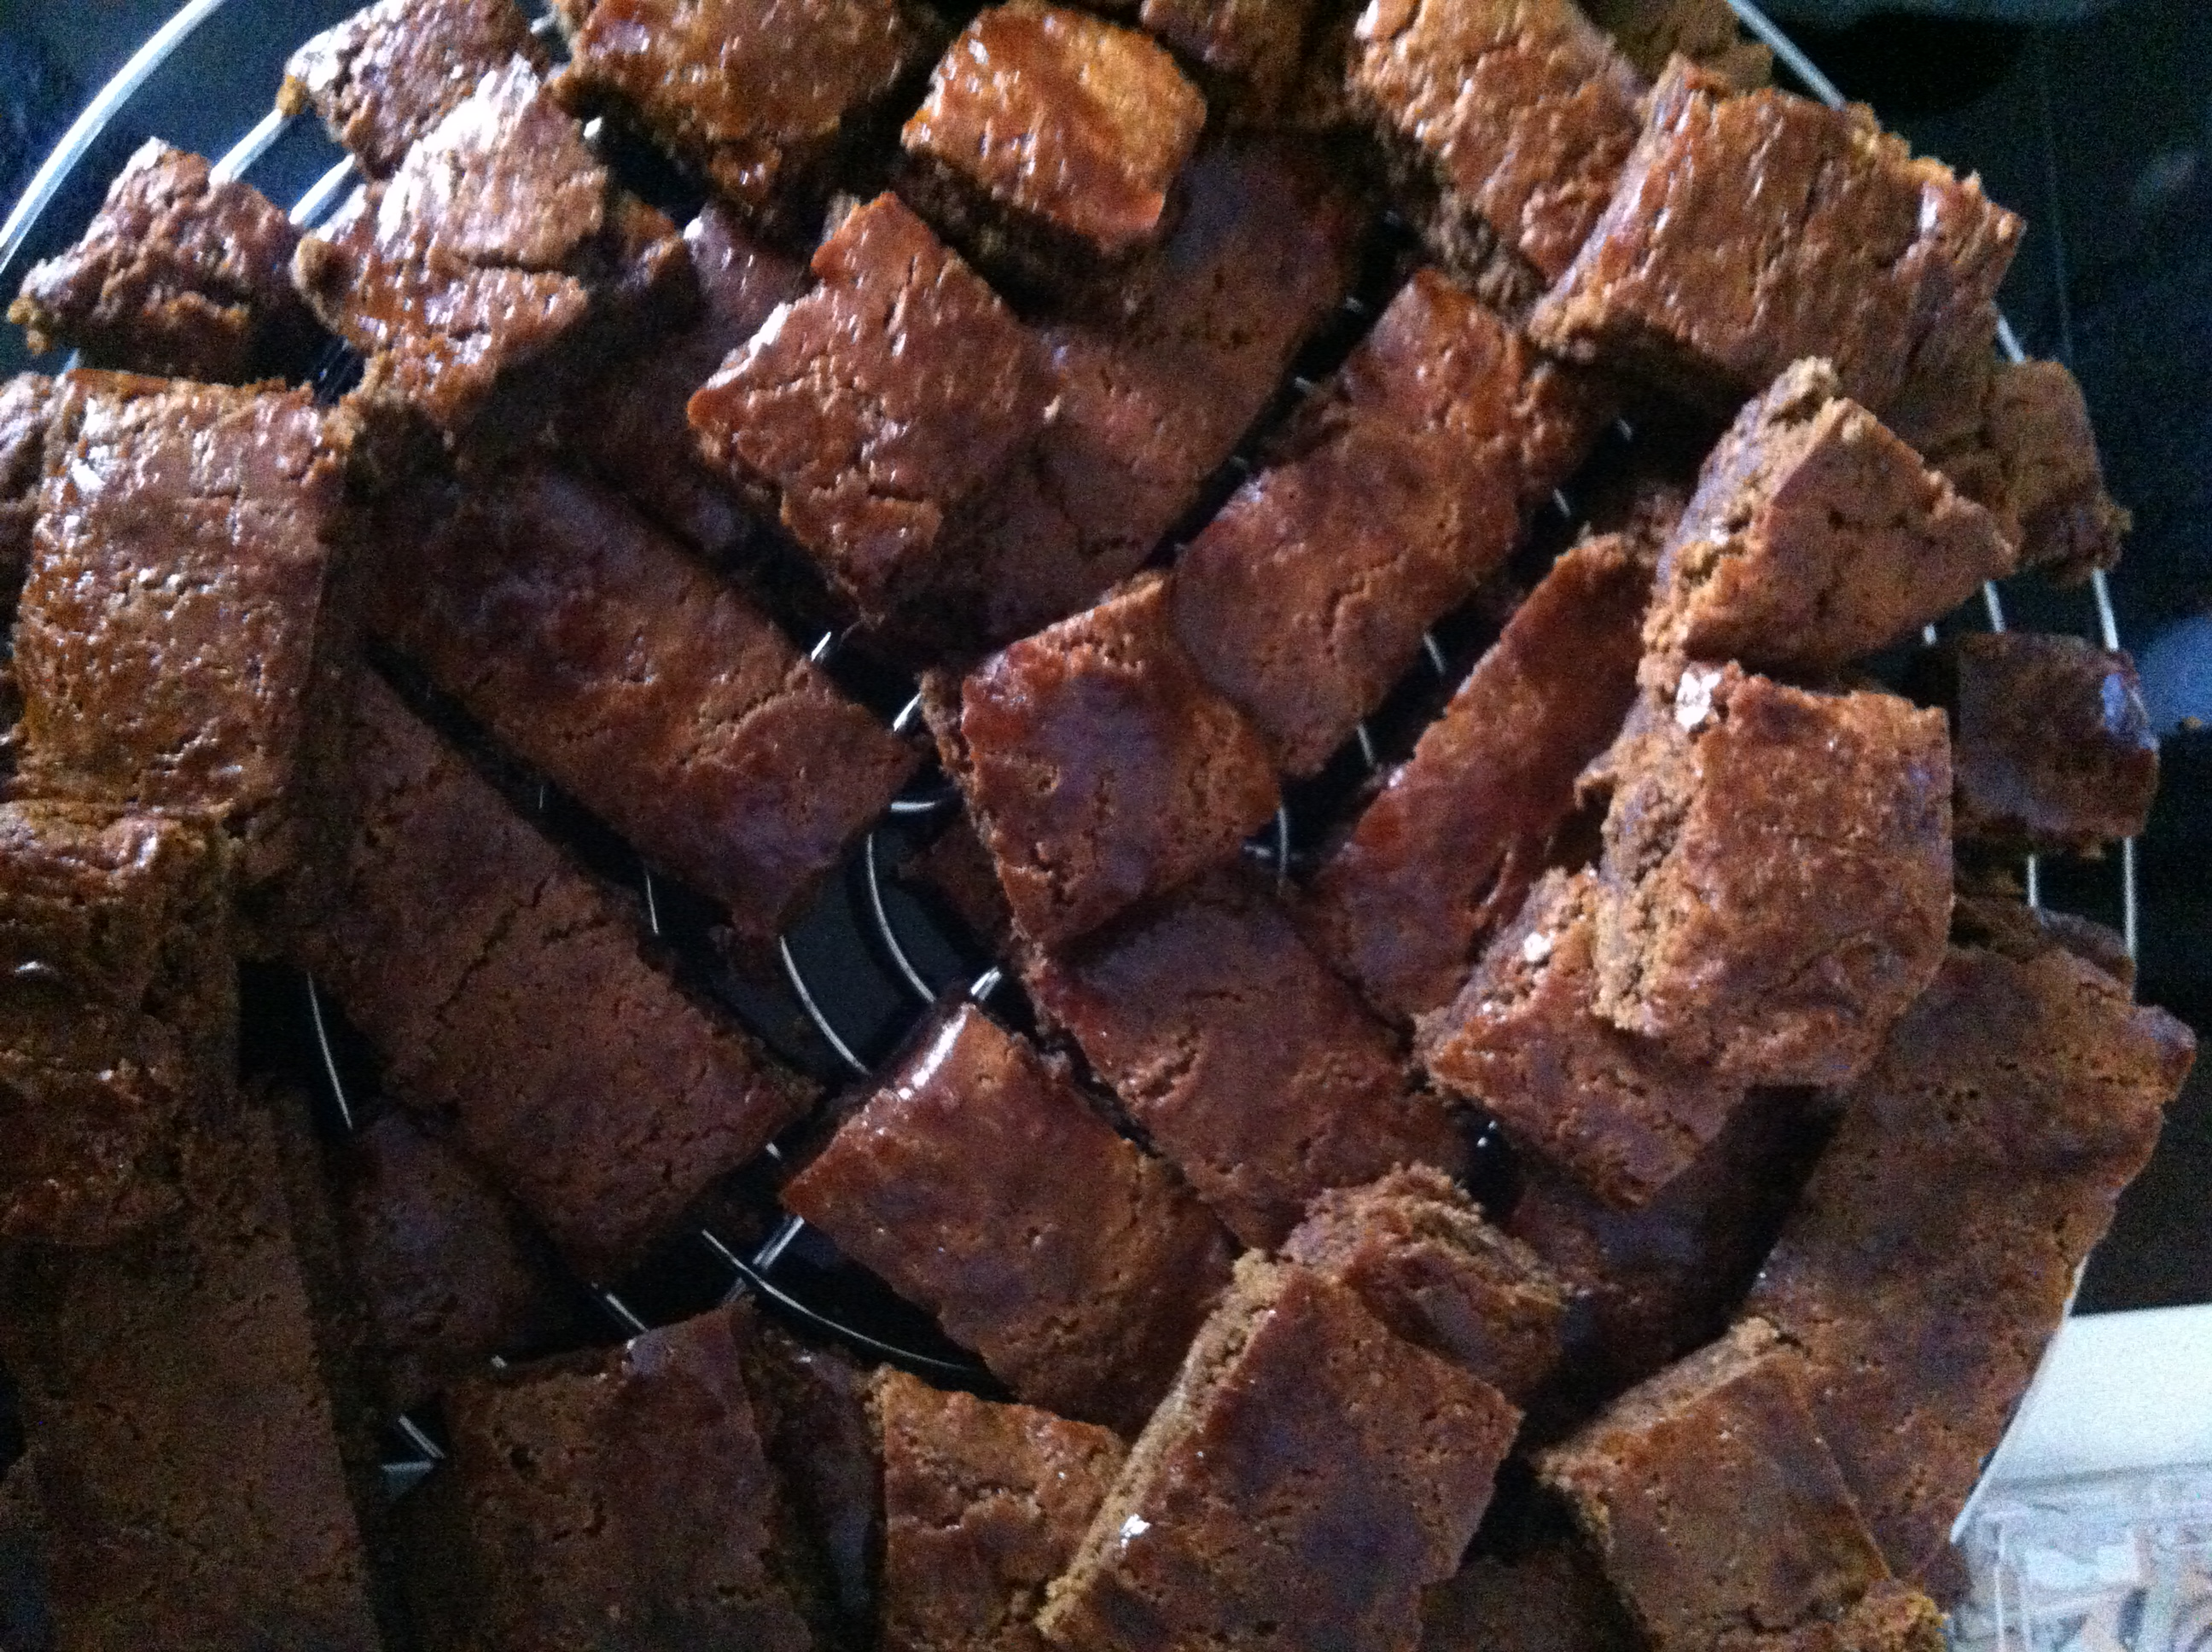
\includegraphics[width=64mm]{Bilder/lebkuchen}}
      
        \ingredient[500]{g}{Mehl}
        \ingredient[100]{g}{Mandeln}
        \ingredient[\fr{1}{2}]{TL}{Zimt}
        \ingredient[\fr{1}{2}]{TL}{Ingwer}
        \ingredient[1]{TL}{geriebene Zitronenschale}
        Alle Zutaten in einer Schüssel gut vermischen.
        \ingredient[1]{TL}{Pottasche}
        \ingredient[2]{EL}{Rosenwasser}
        Pottasche im Rosenwasser auflösen und zu den bereits gemischten Zutaten 
        hinzufügen.
        \ingredient[500]{g}{Sirup}
        \ingredient[100]{g}{Zucker}
        \ingredient[50]{g}{\"Ol}
        Zu der Mehlmasse geben und zu einem festen Teig kneten. \"Uber Nacht an 
        einem warmen Ort stehen lassen. Auf ein gefettetes Backblech ca. 1.5 cm 
        dick ausrollen
        \ingredient[1]{El}{Rosenwasser}
        \ingredient[]{}{Mandeln}
        Teig mit Rosenwasser bestreichen und ggf. mit Mandeln garnieren. Bei 
        150~\degrees C (Gas: Stufe 3) 30 bis 40 Minuten backen.
        \freeform Wenn es schnell gehen muss, muss der Teig nicht 
        zwingenderweise eine ganze Nacht ruhen.
    \end{recipe}

\end{document}
